\begin{figure}[t]
\centering
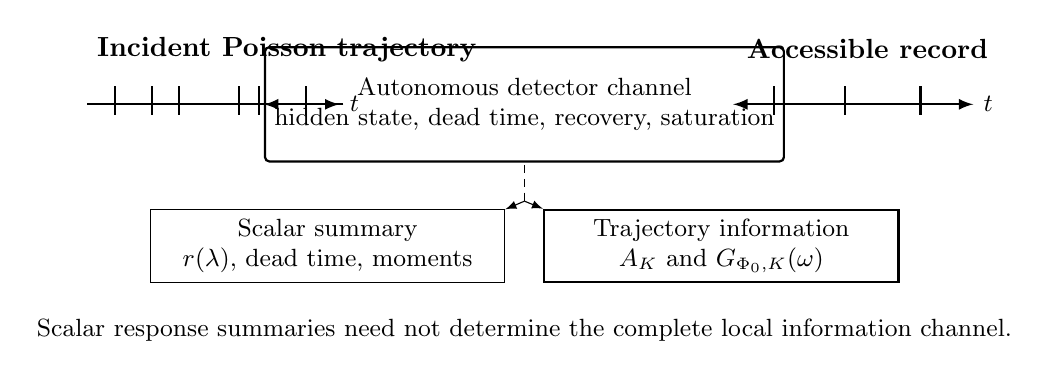
\begin{tikzpicture}[x=1cm,y=1cm,>=latex,font=\small]
  % Input trajectory
  \node[anchor=west,font=\bfseries] at (0,3.25) {Incident Poisson trajectory};
  \draw[->,thick] (0,2.55) -- (3.2,2.55) node[right] {$t$};
  \foreach \x in {0.35,0.82,1.16,1.92,2.18,2.78} {
    \draw[thick] (\x,2.42) -- (\x,2.78);
  }

  % Detector box
  \node[draw,thick,rounded corners=1.5pt,minimum width=4.15cm,minimum height=1.45cm,align=center] (det) at (5.55,2.55)
  {Autonomous detector channel\\hidden state, dead time, recovery, saturation};
  \draw[->,thick] (3.25,2.55) -- (det.west);

  % Output trajectory
  \node[anchor=west,font=\bfseries] at (8.25,3.25) {Accessible record};
  \draw[->,thick] (8.25,2.55) -- (11.25,2.55) node[right] {$t$};
  \foreach \x in {8.72,9.62,10.58} {
    \draw[thick] (\x,2.42) -- (\x,2.78);
  }
  \draw[->,thick] (det.east) -- (8.2,2.55);

  % Two summaries below
  \draw[densely dashed] (5.55,1.78) -- (5.55,1.32);
  \node[draw,minimum width=4.5cm,minimum height=0.9cm,align=center] (scalar) at (3.05,0.75)
  {Scalar summary\\$r(\lambda)$, dead time, moments};
  \node[draw,thick,minimum width=4.5cm,minimum height=0.9cm,align=center] (full) at (8.05,0.75)
  {Trajectory information\\$A_K$ and $G_{\Phi_0,K}(\omega)$};
  \draw[->] (5.55,1.32) -- (scalar.north east);
  \draw[->] (5.55,1.32) -- (full.north west);
  \node[anchor=north,align=center] at (5.55,-0.05)
  {Scalar response summaries need not determine the complete local information channel.};
\end{tikzpicture}
\caption{Trajectory-level formulation. A parameter-independent autonomous detector maps the complete incident Poisson trajectory to an accessible record. Conventional scalar response summaries describe only projections of this channel, whereas the local waveform Fisher operator $A_K$---equivalently its autonomous spectral multiplier $G_{\Phi_0,K}(\omega)$---describes the complete local temporal Fisher metric.}
\label{fig:concept}
\end{figure}
